\chapter{Mixing, Oscillation, Electric Dipole Moments, and Field Operators}

This chapter follows Leonard Susskind's \emph{Advanced Quantum Mechanics} Lecture 8 and is curated by LazyingArt LLC. The lecture begins from a live question about neutrinos, uses that question to build a clean two-state model of mixing, pauses for a long interlude on what an electric dipole moment does and does not tell us about the electron, and then explicitly returns to second quantization. The central theme is simple but powerful: the states in which systems are prepared need not be the states that diagonalize the Hamiltonian. Once that distinction is kept in view, the rest of the lecture unfolds naturally.

\section{Mixing as the Real Issue}

A student asks whether neutrinos, if they have mass, must all have the same mass; if not, how can they mix without violating energy conservation? Susskind's answer is immediate and conceptual. Mass is energy, and the energy eigenstates do not mix with each other. What mixes are the physically named states, the states of \emph{type}. In a schematic notation,
\begin{equation}
|\text{type}\rangle = \sum_n c_n |E_n\rangle .
\end{equation}
Thus the right statement is not that energy eigenstates change into one another, but that the states called ``electron neutrino'' or ``muon neutrino'' need not themselves be energy eigenstates.

He emphasizes that this is a common pattern in quantum mechanics and then says, in effect, that a simple example is enough to see it. The abstract neutrino question is therefore translated into a very concrete one-dimensional problem.

\section{Symmetric Double Well and Approximate Localized States}

Consider a particle moving in a symmetric double-well potential with a high barrier between the two minima. If the barrier were taken to be infinitely high, then the left and right wells would decouple completely. One could solve the left-hand well as though the right-hand well did not exist, and likewise for the right-hand well. The approximate ground-state wavefunctions would then be a left-localized state \(\psi_L\) and a right-localized state \(\psi_R\), both with the same energy \(E\).

In each isolated well the ground state has the familiar qualitative properties: it is smooth, has no nodes, and sits at the lowest possible energy consistent with confinement. Susskind explicitly asks the room to imagine the barrier as a brick wall. It is only a good approximation, but it is a useful one.

\begin{figure}
\centering
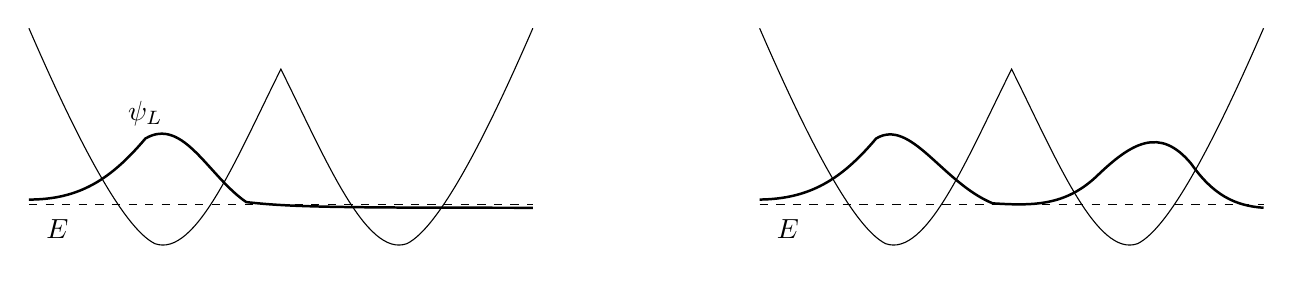
\begin{tikzpicture}[x=0.8cm,y=0.8cm]
\begin{scope}[shift={(-5.8,0)}]
\draw (-4,2.7) .. controls (-3.35,1.2) and (-2.55,-0.45) .. (-2.0,-0.72)
      .. controls (-1.35,-0.95) and (-0.7,0.65) .. (0,2.05)
      .. controls (0.7,0.65) and (1.35,-0.95) .. (2.0,-0.72)
      .. controls (2.55,-0.45) and (3.35,1.2) .. (4,2.7);
\draw[dashed] (-4,-0.10) -- (4,-0.10);
\node at (-3.55,-0.48) {$E$};
\draw[line width=0.9pt] (-4,-0.02) .. controls (-3.2,-0.02) and (-2.7,0.30) .. (-2.15,0.95)
      .. controls (-1.55,1.30) and (-1.15,0.35) .. (-0.55,-0.06)
      .. controls (0.15,-0.14) and (0.9,-0.15) .. (4,-0.15);
\node at (-2.15,1.35) {$\psi_L$};
\end{scope}
\begin{scope}[shift={(5.8,0)}]
\draw (-4,2.7) .. controls (-3.35,1.2) and (-2.55,-0.45) .. (-2.0,-0.72)
      .. controls (-1.35,-0.95) and (-0.7,0.65) .. (0,2.05)
      .. controls (0.7,0.65) and (1.35,-0.95) .. (2.0,-0.72)
      .. controls (2.55,-0.45) and (3.35,1.2) .. (4,2.7);
\draw[dashed] (-4,-0.10) -- (4,-0.10);
\node at (-3.55,-0.48) {$E$};
\draw[line width=0.9pt] (-4,-0.02) .. controls (-3.2,-0.01) and (-2.7,0.30) .. (-2.15,0.95)
      .. controls (-1.6,1.28) and (-1.1,0.25) .. (-0.30,-0.08)
      .. controls (0.35,-0.12) and (0.85,-0.12) .. (1.35,0.35)
      .. controls (1.9,0.88) and (2.35,1.15) .. (2.85,0.55)
      .. controls (3.2,0.05) and (3.55,-0.12) .. (4,-0.15);
\end{scope}
\end{tikzpicture}
\caption{A clean redraw of the opening board sketches. On the left is the one-sided trial state \(\psi_L\), obtained by pretending the barrier is effectively infinite. On the right the same wavefunction has been continued symmetrically through the barrier, illustrating the small but nonzero leakage that eventually produces the true even ground state.}
\end{figure}

Quantum mechanically, however, the barrier is not truly infinite. The wavefunction in the barrier region is not exactly zero; it is only very small. This tiny leakage is the whole story. It is what converts the left-right approximation into a genuine mixing problem.

\section{Parity Eigenstates and Exponential Level Splitting}

At this point Susskind interrupts the naive picture with a theorem: if the potential is symmetric, then the exact energy eigenfunctions can be chosen to be either symmetric or antisymmetric under reflection.

\begin{theorem}
If \(V(x)=V(-x)\) in one dimension, then the eigenfunctions of the Hamiltonian may be chosen to satisfy either
\[
\psi(x)=\psi(-x)
\qquad \text{or} \qquad
\psi(x)=-\psi(-x).
\]
\end{theorem}

Now comes the correction. The one-sided states \(\psi_L\) and \(\psi_R\) are neither symmetric nor antisymmetric, so they cannot be exact eigenstates of the full Hamiltonian. They are only good approximate states when the barrier is high. The true eigenstates are the symmetric and antisymmetric combinations,
\begin{align}
\psi_+ &= \frac{\psi_L+\psi_R}{\sqrt{2}},\\
\psi_- &= \frac{\psi_L-\psi_R}{\sqrt{2}}.
\end{align}
This is exactly how the blackboard notation settles. Susskind then labels the energies by
\begin{align}
H\psi_+ &= (E_1-\epsilon)\psi_+,\\
H\psi_- &= (E_1+\epsilon)\psi_-.
\end{align}
The total splitting is therefore
\begin{equation}
\Delta E = (E_1+\epsilon)-(E_1-\epsilon)=2\epsilon .
\end{equation}

\begin{figure}
\centering
\begin{tikzpicture}[x=1cm,y=1cm]
\draw[->] (0,0) -- (0,3);
\node[left] at (0,2.8) {energy};
\draw (-0.35,1.60) -- (0.35,1.60);
\node[left] at (-0.45,1.60) {$\psi_L,\psi_R$};
\node at (1.7,1.60) {$\Longrightarrow$};
\draw (3.0,1.32) -- (3.75,1.32);
\draw (3.0,1.88) -- (3.75,1.88);
\draw[dashed] (2.8,1.60) -- (3.95,1.60);
\node[right] at (3.9,1.32) {$\psi_+,\ E_1-\epsilon$};
\node[right] at (3.9,1.88) {$\psi_-,\ E_1+\epsilon$};
\node[below] at (3.37,1.60) {$E_1$};
\end{tikzpicture}
\caption{The board logic of the tunnel splitting. The approximate left and right states are nearly degenerate, but the exact symmetric and antisymmetric eigenstates are split by a small amount \(2\epsilon\).}
\end{figure}

The ordering of the levels is part of the lecture's physical point. The symmetric state is slightly lower in energy because it is smoother through the barrier region; allowing the wavefunction to leak and continue symmetrically lowers the energy by a tiny amount. The antisymmetric state is slightly higher because the first excited state in one dimension has one node, and in this symmetric problem that node sits at the midpoint. Extra curvature costs kinetic energy.

Susskind stresses that the effect is very small, exponentially small in the barrier width and height. He does not need an explicit WKB formula here; the important point is that the splitting is real, but tiny. He also remarks that the overall sign of a wavefunction carries no physical information. Replacing \(\psi_-\) by \(-\psi_-\) does not change the state.

\section{Time Evolution and Left-Right Oscillation}

Only after the static picture is clear does Susskind ask the dynamical question: what happens if we start with a particle placed in the left-hand well? This is the decisive step, because oscillation is the time-dependent face of the same mixing phenomenon.

The inverse relations are
\begin{align}
\psi_L &= \frac{\psi_+ + \psi_-}{\sqrt{2}},\\
\psi_R &= \frac{\psi_+ - \psi_-}{\sqrt{2}}.
\end{align}
So an initially left-localized state is
\begin{equation}
\psi(0)=\psi_L=\frac{\psi_+ + \psi_-}{\sqrt{2}}.
\end{equation}
It is not an energy eigenstate, and therefore it must evolve nontrivially.

\begin{remark}
In the lecture the signs in the time-dependent phases briefly wobble, and Susskind explicitly catches the slip. The written notes use the standard Schr\"odinger convention \(e^{-iEt}\). The only physically important quantity here is the relative phase between the two energy eigenstates.
\end{remark}

With that convention,
\begin{equation}
\psi(t)=\frac{1}{\sqrt{2}}\left(e^{-i(E_1-\epsilon)t}\psi_+ + e^{-i(E_1+\epsilon)t}\psi_-\right).
\end{equation}
This is the cleaned version of the board formula. Now factor out the common phase:
\begin{equation}
\psi(t)=\frac{e^{-iE_1 t}}{\sqrt{2}}\left(e^{i\epsilon t}\psi_+ + e^{-i\epsilon t}\psi_-\right).
\end{equation}
At this point the lecture turns from bookkeeping to geometry: one phase runs one way around the unit circle, the other runs the opposite way. The state changes only because these two phases drift out of step.

To see the left-right oscillation explicitly, substitute the definitions of \(\psi_\pm\):
\begin{align}
\psi(t)
&= \frac{e^{-iE_1 t}}{2}
\left[e^{i\epsilon t}(\psi_L+\psi_R)+e^{-i\epsilon t}(\psi_L-\psi_R)\right] \\
&= \frac{e^{-iE_1 t}}{2}
\left[(e^{i\epsilon t}+e^{-i\epsilon t})\psi_L+(e^{i\epsilon t}-e^{-i\epsilon t})\psi_R\right] \\
&= e^{-iE_1 t}\left[\psi_L\cos(\epsilon t)+i\,\psi_R\sin(\epsilon t)\right].
\end{align}
This is the key worked derivation of the chapter. In the two-state approximation, with \(\psi_L\) and \(\psi_R\) orthonormal, the probabilities are
\begin{equation}
P_L(t)=\cos^2(\epsilon t),
\qquad
P_R(t)=\sin^2(\epsilon t).
\end{equation}
So the system oscillates. At intermediate times it is genuinely in superposition; for example, when \(\epsilon t=\pi/4\), the probabilities on the two sides are equal. The lecture insists on this continuity: the phases evolve continuously, and the localization changes continuously with them.

The blackboard derivation isolates the first time at which the relative sign flips. One asks when
\begin{equation}
e^{-i\epsilon t}=-\,e^{i\epsilon t},
\end{equation}
which is the visible milestone on the board. Multiplying through gives
\begin{equation}
e^{2i\epsilon t}=-1.
\end{equation}
For the first occurrence,
\begin{equation}
2\epsilon t=\pi,
\qquad\text{so}\qquad
t_{L\to R}=\frac{\pi}{2\epsilon}.
\end{equation}
At that instant,
\begin{equation}
\psi(t_{L\to R}) \propto \frac{\psi_+-\psi_-}{\sqrt{2}}=\psi_R.
\end{equation}
The overall phase is irrelevant. What matters is that the particle initially placed on the left has evolved into the right-localized state. After another equal interval it swings back again. That is why Susskind says that mixing and oscillation go together.

There is one spoken slip in the lecture immediately after the correct formula: Susskind first says that if \(\epsilon\) is small, the transfer time can be very long, and then momentarily says the opposite. The equation is unambiguous. Small \(\epsilon\) means slow oscillation and a long transfer time.

\section{Neutrino, Ammonia, and Spin Analogies}

With the double well understood, Susskind returns to the original neutrino question. The left and right wells now become a template. In a two-state caricature,
\begin{equation}
|\nu_e\rangle \sim \frac{|m_1\rangle+|m_2\rangle}{\sqrt{2}},
\qquad
|\nu_\mu\rangle \sim \frac{|m_1\rangle-|m_2\rangle}{\sqrt{2}},
\end{equation}
where the mass eigenstates play the role of \(\psi_+\) and \(\psi_-\), and the flavor states play the role of \(\psi_L\) and \(\psi_R\). An electron neutrino is produced in processes involving an electron, just as a particle can be ``plunked'' into the left well. The Hamiltonian, however, evolves the mass eigenstates. As the relative phase accumulates, the same neutrino can later behave as a muon neutrino.

That is the lecture's answer to the apparent conflict with energy conservation: the energy eigenstates do exactly what energy eigenstates are supposed to do. It is the non-energy-eigenstate flavor state that evolves. This is also why oscillation is evidence for neutrino mass. If the neutrino were truly massless, there would be no such mass splitting and no such oscillation phenomenon.

Susskind also discusses ammonia inversion. There the nitrogen atom can sit on one side or the other of the plane of hydrogen atoms, and tunneling through that plane produces the same symmetric and antisymmetric combinations. In ammonia the coupling really is tunneling through a barrier. In the neutrino problem, by contrast, there is no literal barrier in space. There is instead a coupling in the Hamiltonian that mixes electron and muon neutrino states. The mathematics is the same even though the microscopic origin of the coupling is different.

He then says, in effect, that we have already seen this same algebra elsewhere: in spin. Take the two spin states \(|\uparrow_z\rangle\) and \(|\downarrow_z\rangle\). With no field they are degenerate. Now turn on a weak magnetic field in the \(x\)-direction. The energy eigenstates are no longer the \(z\)-eigenstates, but the \(x\)-polarized states. Following the lecture's temporary language,
\begin{align}
|L_x\rangle &= \frac{|\uparrow_z\rangle+|\downarrow_z\rangle}{\sqrt{2}},\\
|R_x\rangle &= \frac{|\uparrow_z\rangle-|\downarrow_z\rangle}{\sqrt{2}}.
\end{align}
These are the direct analogues of \(\psi_+\) and \(\psi_-\). If their energies are \(E\mp\epsilon\), then an initially up spin evolves as
\begin{equation}
|\uparrow_z,t\rangle
= e^{-iEt}\left[\cos(\epsilon t)\,|\uparrow_z\rangle
+ i\sin(\epsilon t)\,|\downarrow_z\rangle\right].
\end{equation}
This is the same formula as for the double well, only now the oscillation is observed as spin precession. After one half period the spin is certainly down; after another half period it is back up. The weakness of the field matters only because it makes the oscillation slow enough to compare with the neutrino story. The mechanism itself does not depend on tunneling. It depends only on off-diagonal mixing in the Hamiltonian.

The lecture briefly notes that real neutrinos involve more than two states: the tau neutrino also mixes in. That makes the algebra more elaborate, but not conceptually different.

\section{Interlude: Electric Dipole Moment, Symmetry, and the ``Electron Sphere'' Claim}

At this point Susskind deliberately changes register. Since the lecture has already drifted into real particle-physics questions, he pauses the formal development and responds to a popular article claiming that a null electron electric-dipole-moment measurement shows that ``the electron is a sphere.'' His view is that this is badly misleading.

\subsection{What was measured?}

What was measured, or rather bounded, is the electric dipole moment of the electron. For separated charges \(\pm q\), the dipole moment is
\begin{equation}
\mathbf d = q\,\boldsymbol{\ell},
\end{equation}
with \(\boldsymbol{\ell}\) the separation vector. A nonzero dipole moment means that the charge distribution is displaced relative to some center.

For the electron, however, the relevant question is not merely whether the charge is off-center in some arbitrary direction. The electron has spin and therefore an axis. It also has a magnetic moment. The physically meaningful question is whether there is a correlation between the displacement of charge and that axis:
\begin{equation}
\mathbf d_e \parallel \boldsymbol{\mu}_e
\qquad \text{or equivalently} \qquad
\mathbf d_e \parallel \mathbf S .
\end{equation}
That is what Susskind means by the electron's electric dipole moment. Conceptually, one asks whether placing the spin in an electric field would split the two orientations:
\begin{equation}
\Delta E_{\mathrm{EDM}}=-\mathbf d_e\cdot \mathbf E .
\end{equation}
The actual tabletop experiment is more subtle than this elementary picture, but this is the basic idea.

\subsection{Why no EDM does not mean sphere}

The first correction is elementary. A body can have no dipole moment and still not be spherical. An ellipsoid, for example, can have zero dipole moment and yet carry a quadrupole moment. One can also imagine higher multipoles with no dipole and no quadrupole. So the statement ``no EDM'' does not by itself even come close to proving ``sphere.''

Susskind then turns the argument into a quantum-mechanical one. Imagine a lopsided dumbbell-like molecule. Classically it certainly does not look spherical. But if its ground state has angular momentum zero, then because angular momentum generates rotations,
\begin{equation}
J=0 \qquad \Longrightarrow \qquad \text{rotationally invariant ground state.}
\end{equation}
So the quantum state can be rotationally symmetric even though the underlying object is not a classical sphere. One may think of the state as a superposition of all orientations.

This immediately raises a measurement question. A quick snapshot of orientation is itself a measurement of angle. Such a measurement forces the system into a state of definite orientation, and therefore kicks its angular momentum. Susskind presents this as the angular-momentum version of the ordinary position-momentum uncertainty principle. Whether the lopsidedness can actually be resolved depends on the energy needed to excite rotational states. For a macroscopic dumbbell that energy spacing is tiny, so ordinary probes can resolve orientation. For a tightly bound microscopic system, the spacing can be so large that ordinary probes only see the rotationally averaged state.

The lecture pushes this point all the way to hadronic scales. A meson, thought of loosely as a two-body dumbbell, may look spherical to low-energy probes because the energy required to excite rotational structure is extremely large. ``Sphere or not'' therefore becomes a question about the resolving power of the experiment.

Susskind then makes a sharper point about the electron. Independently of any EDM measurement, the electron is a spin-\(\tfrac12\) particle. It has an axis. It has a magnetic moment. In that very direct sense it is already not a spherically symmetric scalar object. So the slogan that the electron ``is a sphere'' was, in his view, already wrong before one even began discussing the EDM bound.

\subsection{Parity and time reversal}

The real content of the EDM discussion is symmetry. Under parity, an electric dipole moment behaves as an ordinary polar vector, while a magnetic moment behaves as an axial vector:
\begin{align}
P:\qquad &\mathbf d_e \to -\mathbf d_e,
&\boldsymbol{\mu}_e \to \boldsymbol{\mu}_e .
\end{align}
Under time reversal, the circulating current that defines the magnetic moment reverses, but a static electric displacement does not:
\begin{align}
T:\qquad &\mathbf d_e \to \mathbf d_e,
&\boldsymbol{\mu}_e \to -\boldsymbol{\mu}_e .
\end{align}
Therefore a nonzero EDM aligned with the electron's spin axis is forbidden by exact parity symmetry and also by exact time-reversal symmetry:
\begin{equation}
(P\ \text{exact}) \Rightarrow \mathbf d_e=0,
\qquad
(T\ \text{exact}) \Rightarrow \mathbf d_e=0.
\end{equation}

This is precisely the logic Susskind tries to draw geometrically on the board. Under mirror reflection, the magnetic axis is reproduced with the same orientation, whereas a displaced charge distribution would reverse its relation to that axis. If the world had exact left-right symmetry and there were only one kind of electron, the mirrored electron would have to be the same electron, and the only consistent possibility would be zero EDM. Under time reversal the current reverses, and hence the magnetic moment flips, while the displaced charge does not. The same conclusion follows again.

Now parity is not a good symmetry of the weak interactions, so parity alone does not save us. But time-reversal violation in the standard model is extremely small, and so the standard-model electron EDM is correspondingly tiny. The experiment he is discussing did not detect any EDM. That is not evidence that the electron is spherical. It is evidence that any EDM is very strongly suppressed, which is good for the standard model and constraining for possible extensions beyond it.

The lecture's punchline is therefore careful and modest: the null result says the electron does not have an observable electric dipole moment at the measured level. It does not say the electron is a sphere.

\section{Return to Second Quantization: Fourier Transforms, Momentum Modes, and Locality}

After the break Susskind explicitly restarts the main thread: ``we were doing second quantization.'' He does so gently, beginning with ordinary Fourier transforms in single-particle quantum mechanics and then lifting the same structure to field operators.

\subsection{From \(\psi(x)\) to \(\tilde{\psi}(p)\)}

He first reminds the class that little \(\psi\), not capital \(\Psi\), is the wavefunction of a single particle. In position space,
\begin{equation}
P(x)=|\psi(x)|^2
\end{equation}
is the probability density to find the particle at position \(x\). The momentum-space wavefunction is its Fourier transform,
\begin{equation}
\tilde{\psi}(p)=\int dx\,\psi(x)\,\frac{e^{-ipx}}{\sqrt{2\pi}},
\end{equation}
and the inverse relation is
\begin{equation}
\psi(x)=\int dp\,\tilde{\psi}(p)\,\frac{e^{ipx}}{\sqrt{2\pi}}.
\end{equation}
Then
\begin{equation}
P(p)=|\tilde{\psi}(p)|^2
\end{equation}
is the probability density for momentum \(p\).

For a free particle,
\begin{equation}
H=\frac{p^2}{2m},
\end{equation}
so momentum eigenstates are also energy eigenstates, and their position-space wavefunctions are plane waves,
\begin{equation}
\psi_p(x)\propto e^{ipx}.
\end{equation}
This is the point of departure for the second-quantized version.

\subsection{Field operators in position and momentum space}

Susskind then goes back to the field operator. On the blackboard he writes the annihilation and creation pieces as \(\Psi_-(x)\) and \(\Psi_+(x)\). Keeping that notation for a moment,
\begin{align}
\Psi_-(x) &= \sum_i a_i\,\psi_i(x),\\
\Psi_+(x) &= \sum_i a_i^\dagger\,\psi_i^*(x).
\end{align}
Here \(\psi_i(x)\) is the ordinary one-particle wavefunction of the \(i\)-th mode, while \(a_i\) and \(a_i^\dagger\) annihilate and create particles in that mode. From this point on it is convenient to rename
\[
\Psi(x)\equiv \Psi_-(x),
\qquad
\Psi^\dagger(x)\equiv \Psi_+(x).
\]

For a free particle the discrete mode label \(i\) is replaced by the continuous momentum label \(p\). Using the plane waves \(e^{ipx}\), one obtains the standard reconstructed formulas
\begin{align}
\Psi(x) &= \int \frac{dp}{\sqrt{2\pi}}\,a(p)\,e^{ipx},\\
\Psi^\dagger(x) &= \int \frac{dp}{\sqrt{2\pi}}\,a^\dagger(p)\,e^{-ipx}.
\end{align}
These are the field-operator analogues of the ordinary Fourier transform. They can be inverted exactly as before:
\begin{align}
a(p) &= \int \frac{dx}{\sqrt{2\pi}}\,\Psi(x)\,e^{-ipx},\\
a^\dagger(p) &= \int \frac{dx}{\sqrt{2\pi}}\,\Psi^\dagger(x)\,e^{ipx}.
\end{align}
The normalization in this part of the live lecture is not completely legible on the board, but the standard \(1/\sqrt{2\pi}\) convention is the natural cleaned reconstruction.

The conceptual content is straightforward. \(\Psi^\dagger(x)\) creates a particle at position \(x\), while \(a^\dagger(p)\) creates a particle with momentum \(p\). Position-space and momentum-space creation operators are Fourier conjugates of one another, just as \(\psi(x)\) and \(\tilde{\psi}(p)\) are Fourier conjugates in ordinary quantum mechanics.

\subsection{Bosonic commutators and the independence of separated measurements}

The lecture then turns to commutators. For bosons,
\begin{equation}
[a_i,a_j^\dagger]=\delta_{ij},
\qquad
[a_i,a_j]=0,
\qquad
[a_i^\dagger,a_j^\dagger]=0.
\end{equation}
The continuum version is
\begin{equation}
[a(p),a^\dagger(p')]=\delta(p-p').
\end{equation}
Now compute the equal-time field commutator from the discrete expansion:
\begin{align}
[\Psi(x),\Psi^\dagger(y)]
&= \sum_{i,j}\psi_i(x)\psi_j^*(y)\,[a_i,a_j^\dagger] \\
&= \sum_i \psi_i(x)\psi_i^*(y) \\
&= \delta(x-y),
\end{align}
where the last step uses completeness of the one-particle basis. Likewise,
\begin{equation}
[\Psi(x),\Psi(y)]=0,
\qquad
[\Psi^\dagger(x),\Psi^\dagger(y)]=0.
\end{equation}

Susskind emphasizes that the most important point is not that \(\Psi\) is non-Hermitian. One can always take real and imaginary parts to obtain Hermitian combinations. The important point is the delta function. When \(x\neq y\), the commutator vanishes. Measurements of the field at different points therefore do not interfere with one another. When \(x=y\), the nontrivial commutator reappears, and the same-point real and imaginary parts cannot be measured simultaneously without mutual disturbance.

This is the lecture's locality heuristic in bosonic second quantization. Commuting operators at separated points express the independence of separated measurements. Susskind presses this toward a relativistic intuition: if measurements at spacelike separated points failed to commute, one would seem to have a mechanism by which a measurement here gives a kick there. In the lecture he uses this to answer a question about entanglement. Correlation is not influence. The vanishing commutator at separated points is exactly what prevents the formalism from turning entanglement into superluminal causal action.

He ends by looking ahead. Fermions will not satisfy these commutators; they satisfy anticommutation relations instead. That sounds alarming if one tries to interpret the fermion field itself as a directly measurable local observable. The resolution, postponed to the next lecture, is that fermion fields are not observables in the same direct sense as bosonic fields.

\section{Summary}

The lecture begins with a neutrino puzzle but quickly reveals a much broader lesson. Energy eigenstates do not mix; the prepared states do. In the symmetric double well this distinction is visible on the board: the approximate left and right states are not exact eigenstates, the exact eigenstates are the symmetric and antisymmetric combinations, and the tiny splitting between them drives left-right oscillation.

Susskind then shows that the same algebra reappears in neutrino oscillation, ammonia inversion, and spin precession. The long EDM interlude serves a different purpose: it disentangles a symmetry statement from a careless popular slogan. A null electron EDM measurement does not prove that the electron is spherical; it shows only that any EDM is strongly suppressed. Finally, returning to second quantization, the lecture replays the familiar Fourier-transform structure at the operator level and ends with the bosonic equal-time commutator, whose main physical meaning is the independence of measurements at different points. The next lecture, by design, begins where this one stops: with fermions and anticommutators.